\documentclass[border=1mm]{standalone}
% \usepackage[margin=2.5cm]{geometry}

\usepackage{graphicx,tikz,tikz-layers,amsmath,ifthen,tabularray} 
\usetikzlibrary{decorations.markings,calc,positioning,arrows,shapes.geometric,arrows.meta,matrix}

\colorlet{myred}{red!80!black}
\colorlet{myblue}{blue!80!black}
\colorlet{mybluee}{myblue!80!black}
\colorlet{mygreen}{green!60!black}
\colorlet{myorange}{orange!70!red!60!black}
\colorlet{mydarkred}{red!20!black}
\colorlet{mydarkblue}{blue!40!black}
\colorlet{mydarkgreen}{green!20!black}




\begin{document}

% \resizebox{\textwidth}{!}{
\tikz[font=\footnotesize, scale=1, every node/.style={outer sep=0pt, inner sep=0pt, align=center, rounded corners=.5mm}, w/.style={minimum width=#1}, h/.style={minimum height=#1}, s/.style={minimum size=#1}, eu/.style={shorten >=#1}, ed/.style={shorten <=#1}, line join=round]
{
\tikzset{>={Latex[length=1.5mm, width=1.25mm]}}

\node[draw, w=2cm, h=.8cm, fill=myred!15] (ep) {Embedded\\Patches};
\node[draw, w=2cm, h=.5cm, fill=myblue!15, above=.65cm of ep] (norm1) {Norm};
\node[draw, w=2cm, h=.8cm, fill=mygreen!15, above=.45cm of norm1] (mha) {Multi-Head\\Attention};
\node[draw, circle, s=.3cm, above=.25cm of mha] (plus1) {$+$};
\node[draw, w=2cm, h=.5cm, fill=myblue!15, above=.25cm of plus1] (norm2) {Norm};
\node[draw, w=2cm, h=.5cm, fill=orange!20, above=.35cm of norm2] (mlp) {MLP};
\node[draw, circle, s=.3cm, above=.25cm of mlp] (plus2) {$+$};

\begin{scope}[on behind layer]
\node[draw, w=2.6cm, h=4.9cm, fill=blue!50!cyan!15, anchor=south] (box) at ([yshift=-.35cm]norm1.south) {};    
\end{scope}

% Wide blue rectangle
\node[draw, w=10cm, h=.7cm, fill=blue!50!cyan!15, left=1cm of box.west] (rec1) {Transformer Encoder};
\node[draw, w=5cm, h=.7cm, fill=orange!20, above=0.6cm of rec1] (mlphead) {MLP Head};
\node[draw, w=8.6cm, h=.5cm, fill=myred!15, anchor=south east] (rec2) at ([yshift=-2cm]rec1.south east) {Linear Projection of Flattened Patches};

% Small ellipse-like shapes
\node[draw, w=.3cm, h=.6cm, rounded corners=1mm, anchor=east, fill=myred!15] (1) at ([xshift=-.25cm]$(rec1.south east)!.5!(rec2.north east)$) {};

\foreach \i[count=\j] in {2,3,...,10}
\node[draw, w=.3cm, h=.6cm, rounded corners=1mm, anchor=east, fill=myred!15, left=.68cm of \j] (\i)  {};

\node at (10) {*};

\foreach \i[count=\j] in {9,...,1}
\node[draw, w=.3cm, h=.6cm, rounded corners=1mm,  fill=mydarkblue!15, left=0cm of \i]  {\j};

\node[draw, w=.3cm, h=.6cm, rounded corners=1mm,  fill=mydarkblue!15, left=0cm of 10] (00)  {0};


\node[draw, draw = white, s=1cm, anchor=south west, fill=white] (mlph) at ([yshift=.5cm]rec1.north west) {};
\node[draw, draw = white, left=.5cm of mlph, inner sep=2mm, rounded corners=3mm, fill=white] (class) {\color{white}\rotatebox{90}{Classification}};

\node[left=.5cm of plus2] {$n\times$};
\node[s=1.5cm, anchor=north west] (photo) at ([yshift=-2.4cm]class.south west) {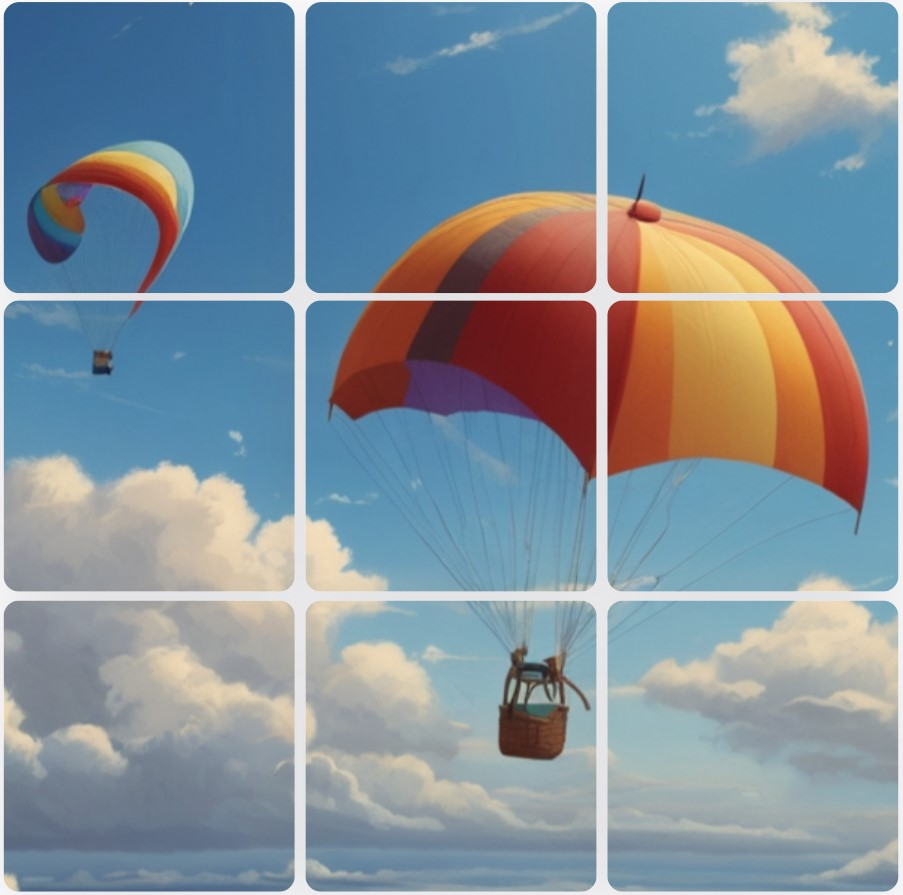
\includegraphics[width=1.5cm]{images/mosaic1/balloon.jpg}};

\node[anchor=north west] (im1) at ([yshift=-.5cm]rec2.south west) {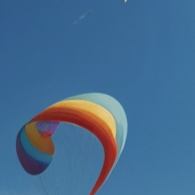
\includegraphics[width=.75cm]{images/mosaic1/1.png}};

\foreach \i[count=\j] in {2,3,...,9}
\node[right=.23cm of im\j] (im\i) {\includegraphics[width=.75cm]{images/mosaic1/\i.png}};

% Arrows and labels
\draw[] (ep)--coordinate[pos=.7] (a) (norm1);
\draw[->] (norm1)--coordinate[pos=.35] (b) (mha);
\draw[->] (b)-|(mha.-30);
\draw[->] (b)-|(mha.210);
\draw[] (mha)--(plus1);
\draw[] (plus1)--coordinate[pos=.5] (c) (norm2);
\draw[->] (norm2)--(mlp);
\draw[] (mlp)--(plus2);
\draw[->] (plus2)--node[pos=1, above=1mm] (te) {\textbf{Transformer Encoder}} +(0,.5);

\draw[->, rounded corners=1mm] (a)--++(1.15,0) |- (plus1);
\draw[->, rounded corners=1mm] (c)--++(1.15,0) |- (plus2);

\foreach \i in {1,2,...,10}{
  \draw[->] (\i)--(\i|-rec1.south);
  \ifnum\i=10
  \else
    \draw (\i)--(\i|-rec2.north);
  \fi
}


\draw[<-] (mlphead)--(mlphead|-rec1.north);
\draw[->] (mlphead.north) -- +(0,0.7);
\draw[<-] (im1.west)--(im1.west-|photo.east);
\draw[<-] (00)--node[pos=1, left=-1mm, align=left, font=\tiny] {Patch $+$\\Position\\Embedding} +(-.5,0);

\tikzset{>={Latex[length=3.2mm, width=2.25mm]}}
% \draw[ultra thick, gray] (rec1)--(rec1-|box.west);

\node[xshift=0.48cm] at (rec1.east) {\textbf{=}};

\node at ([xshift=0cm]rec1|-te) {\textbf{Vision Transformer (ViT)}};


}

% }



\end{document}
